\documentclass[../report]{subfiles}
\setcounter{section}{0}
\begin{document}

本章では,「ふーろぐ」について説明する.
\bunseki{頼亜弥}

\section{ふーろぐの概要}
本グループが開発した「ふーろぐ」の概要について以下にて説明する.補足として,撮影者は一人暮らしの高齢者に当たる.

まず,撮影者にはこのようなボックスを自宅に置いていただく(図\ref{fig:box}).
\begin{figure}[htbp]
    \begin{center}
        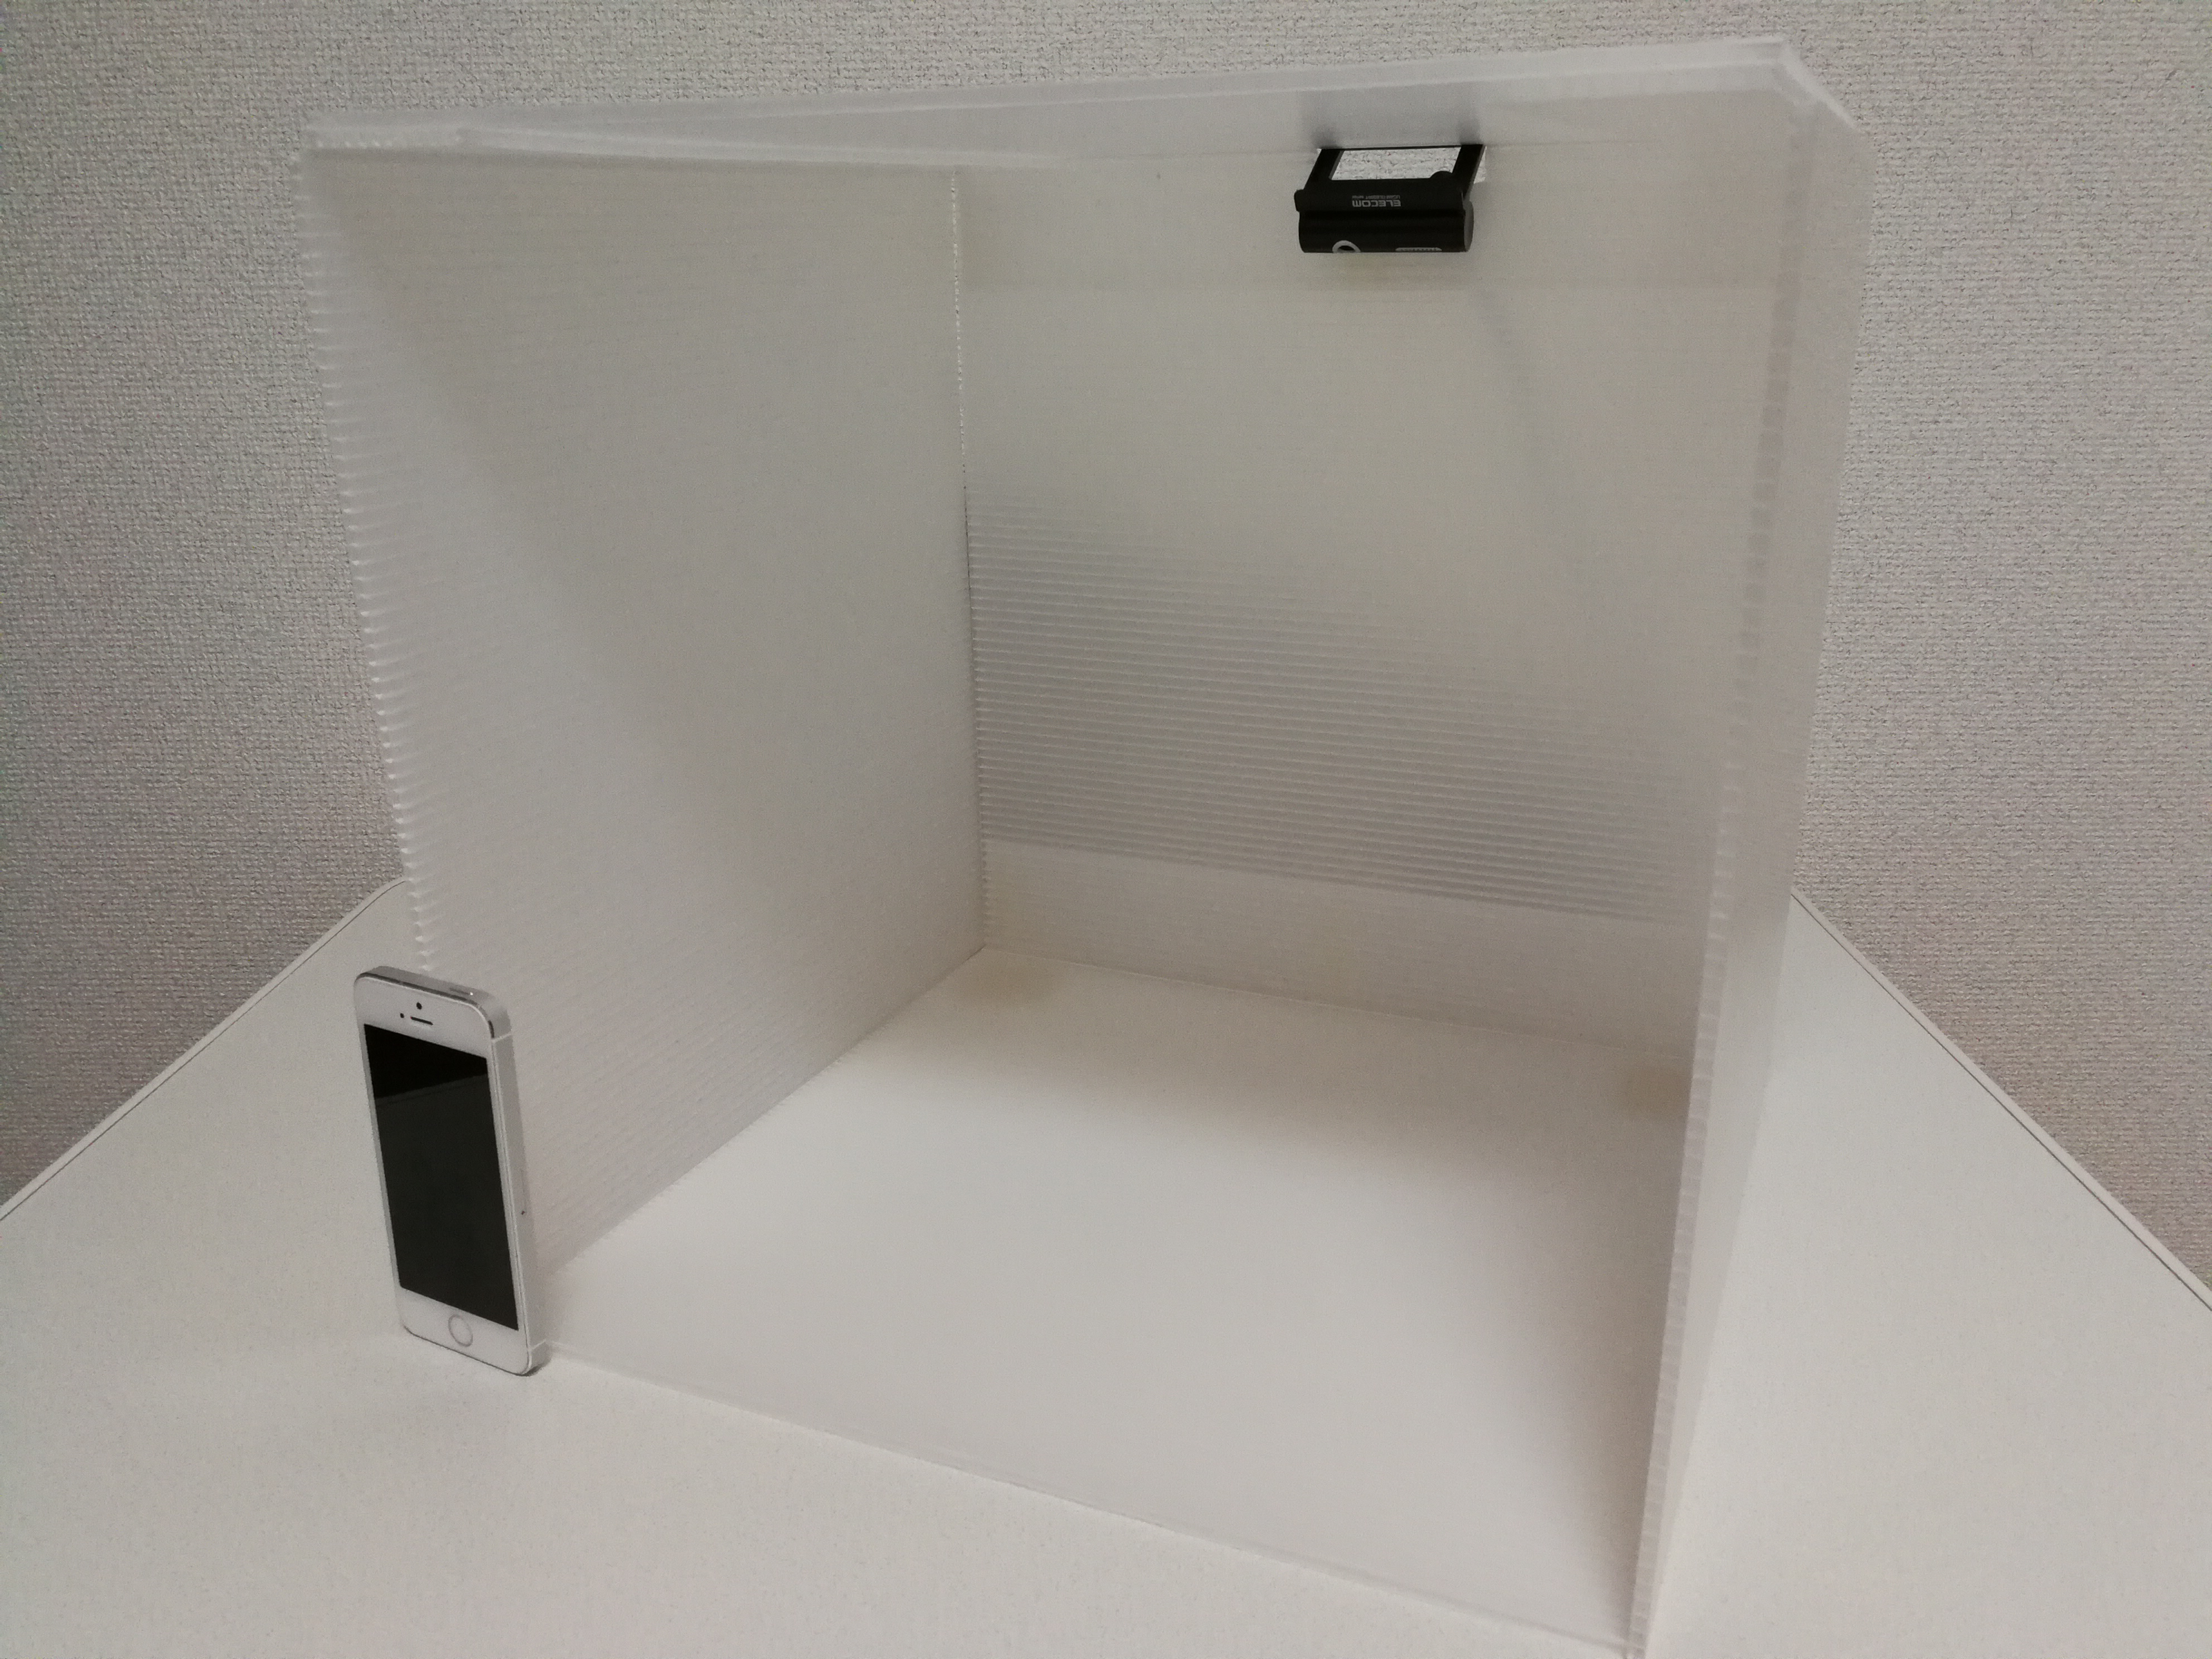
\includegraphics[width=10cm]{imgs/5_box.jpg}
        \caption{ボックス}
        \label{fig:box}
    \end{center}
\end{figure}
\bunseki{頼亜弥}

\section{ふーろぐのポイント}
本グループが開発した「ふーろぐ」のポイントとして三つ挙げられる.

1つ目は,食生活を簡単に記録できることである.
撮影者は,料理をボックスの中に置くという簡単な動作だけで,料理の写真を撮影することができる.
撮影された料理の写真は自動でサーバーに送信され,蓄積されてていく仕組みとなっている.
また,撮影者は自宅にあるテレビを通して料理の写真を閲覧することができる.

2つ目は,離れて暮らす家族とのコミュニケーション支援ができることである.
撮影者は撮影した料理の写真を家族と共有することができる.
家族は料理の写真に対し,アドバイスやフィードバックなどを撮影者に向けて送信することができる.
撮影者は家族からのメッセージをテレビにて閲覧することができる.
撮影者は家族からのメッセージを閲覧することで,食生活に対する意識が変わることが期待できる.また,家族とのコミュニケーションのきっかけにもなる.

3つ目は,一人暮らしの高齢者に対する見守り支援になることである.
家族は撮影者の料理の写真を毎日閲覧することで,撮影者の食生活を知ることができる.
また,撮影者と離れて暮らしていても,食生活を通して撮影者見守ることができる.
\bunseki{頼亜弥}

\section{ふーろぐの使い方}
ここでは,「ふーろぐ」の使い方を「ボックス」,「Web画面」,「テレビ画面」に分けて説明する.補足として,撮影者は一人暮らしの高齢者に当たる.
\bunseki{頼亜弥}

\subsection{ボックス}
撮影者は日々の料理をボックスの中に置くことで,料理の写真が自動で撮影される(図\ref{fig:fl}).
撮影者は自宅にあるテレビ画面にて,撮影された写真を閲覧することができる.
\begin{figure}[htbp]
    \begin{center}
        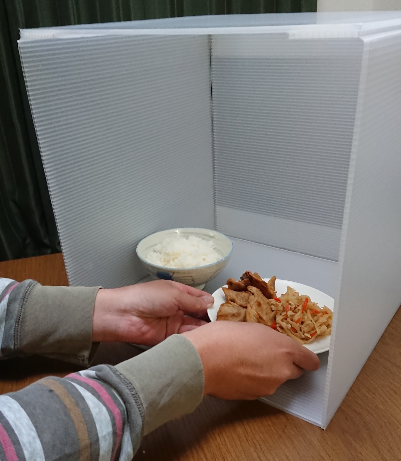
\includegraphics[height=10cm]{imgs/5_fl.png}
        \caption{ふーろぐ}
        \label{fig:fl}
    \end{center}
\end{figure}
\bunseki{頼亜弥}

\subsection{Web画面}
ここでは, 撮影者の家族と医療従事者が閲覧することができるWeb画面について説明する.
\bunseki{山根春貴}

\subsubsection{撮影者管理画面}
管理している撮影者を表示する画面である(図\ref{fig:5_dashboard}).
閲覧者が無駄な操作をしないために撮影者が最後に撮影した時間を表示している.
管理している撮影者をクリックするとカレンダー画面に遷移する.
\begin{figure}[htbp]
    \begin{center}
        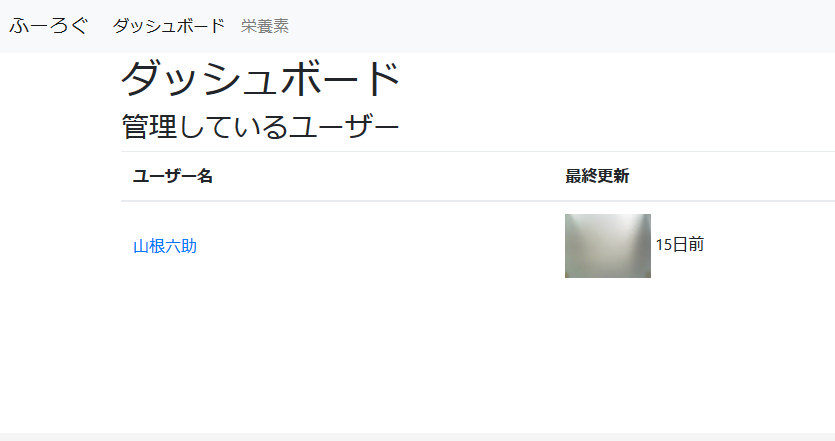
\includegraphics[width=10cm]{imgs/5_dashboard.png}
        \caption{撮影者管理画面}
        \label{fig:5_dashboard}
    \end{center}
\end{figure}
\bunseki{山根春貴}

\subsubsection{カレンダー画面}
対象の撮影者のカレンダー画面である(図\ref{fig:calendar-month}).
カレンダーの日をクリックするとその日のデイリー画面に遷移する.

\begin{figure}[htbp]
    \begin{center}
        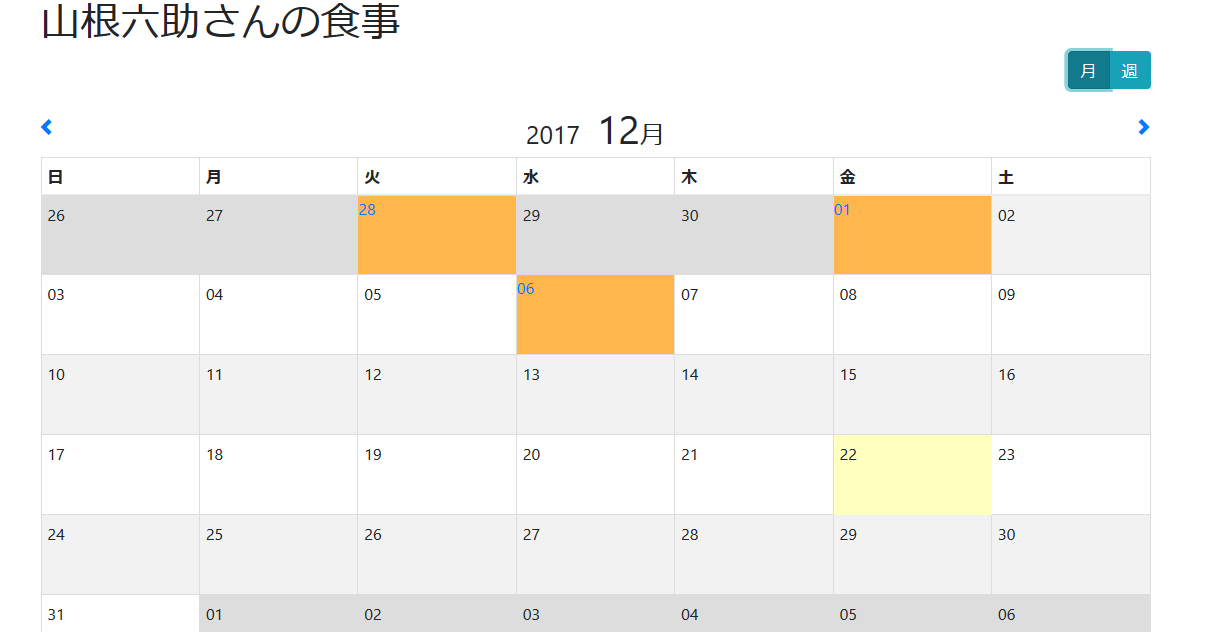
\includegraphics[width=10cm]{imgs/5_month.png}
        \caption{カレンダー画面(月表示)}
        \label{fig:calendar-month}
    \end{center}
\end{figure}

また, 「月表示」だけではなく「週表示」に変更することも可能で, 「週表示」の画面は, 対応した日に撮影された写真が表示される(図\ref{fig:calendar-week}).

\begin{figure}[htbp]
    \begin{center}
        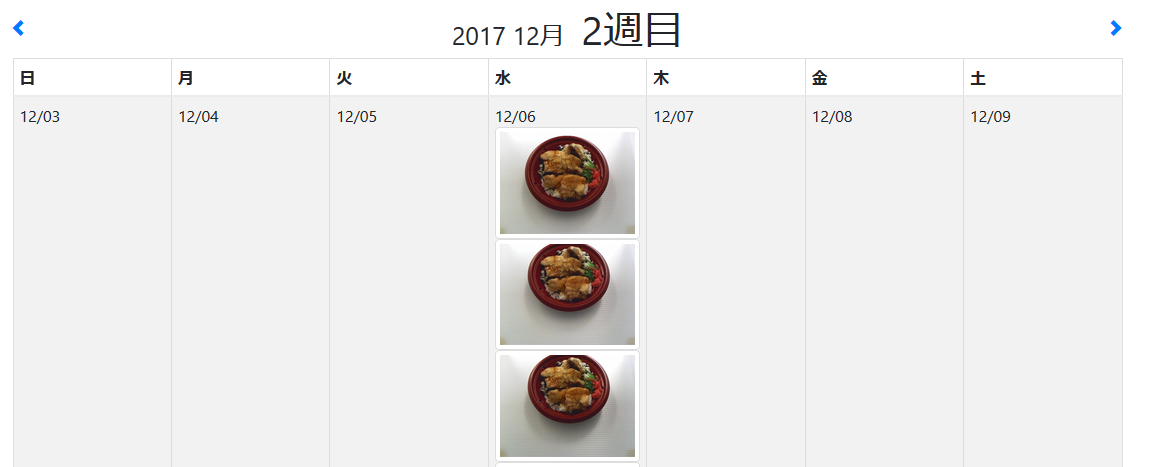
\includegraphics[width=10cm]{imgs/5_week.png}
        \caption{カレンダー画面(週表示)}
        \label{fig:calendar-week}
    \end{center}
\end{figure}
\bunseki{山根春貴}

\subsubsection{デイリー画面}
対応した日に撮影された写真と料理名が表示される(図\ref{fig:meal}).

\begin{figure}[htbp]
    \begin{center}
        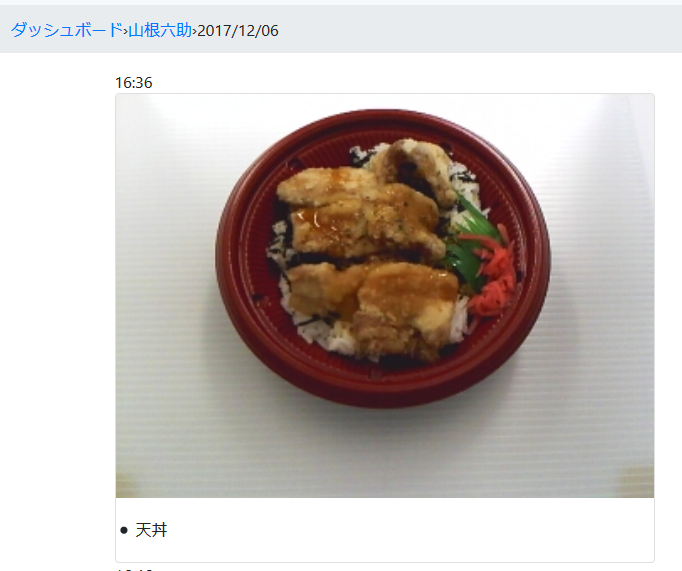
\includegraphics[width=10cm]{imgs/5_day1.png}
        \caption{撮影された料理と料理名}
        \label{fig:meal}
    \end{center}
\end{figure}

また, レーダーチャートも表示している(図\ref{fig:radar}).

\begin{figure}[htbp]
    \begin{center}
        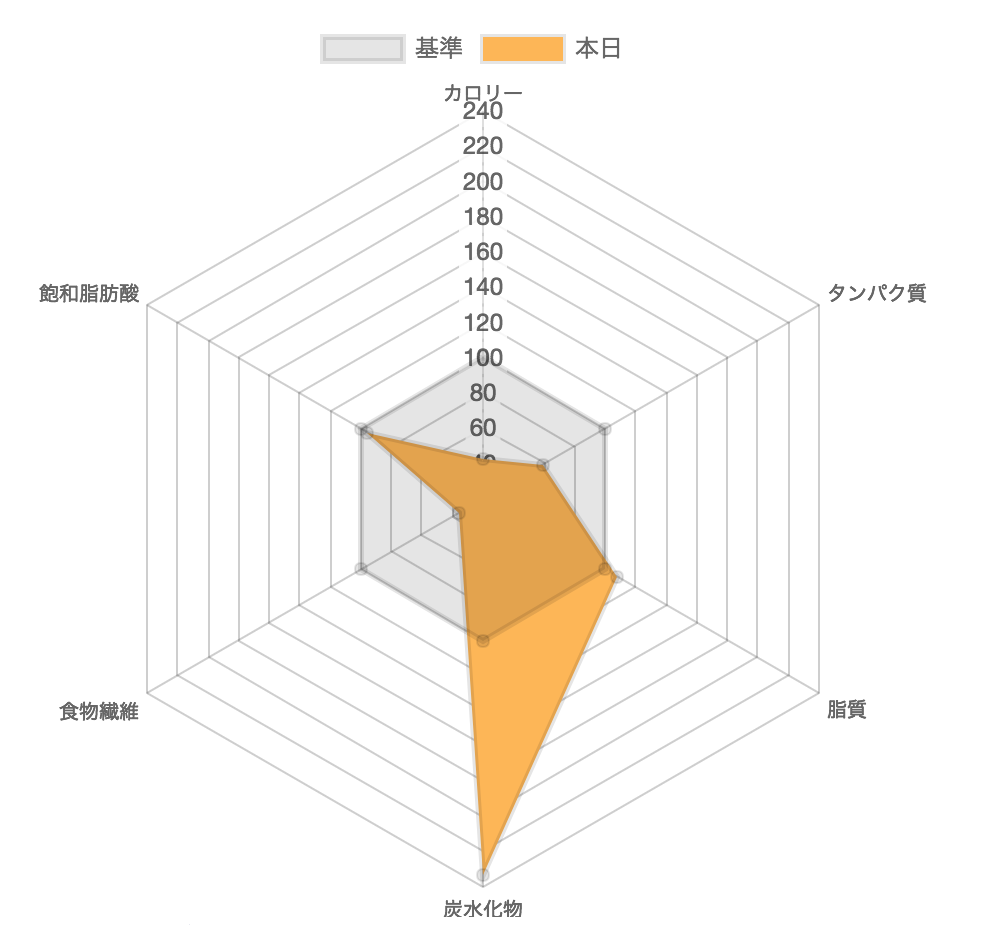
\includegraphics[width=8cm]{imgs/6_radar.png}
        \caption{栄養価のレーダーチャート}
        \label{fig:radar}
    \end{center}
\end{figure}

これらの情報から撮影者に対してメッセージ画面を送信することができるようになっている(図\ref{fig:message}).
メッセージを送信するとテレビ画面に送信したメッセージが表示される.

\begin{figure}[htbp]
    \begin{center}
        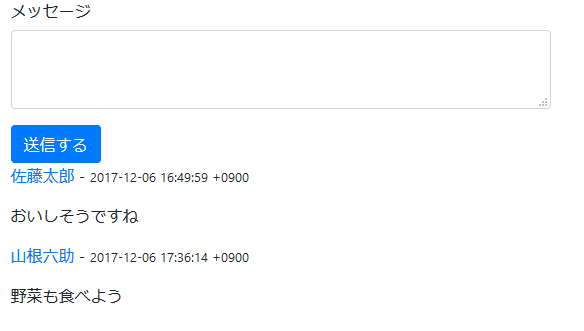
\includegraphics[width=10cm]{imgs/5_day3.png}
        \caption{メッセージ機能}
        \label{fig:message}
    \end{center}
\end{figure}
\bunseki{山根春貴}

\subsection{テレビ画面}
ここでは撮影者が閲覧することができるテレビ画面について説明する.
撮影者がICTに不慣れでも扱いやすく操作がいらないように, 一画面に機能を収めている(図\ref{fig:tv-all}).
\begin{figure}[htbp]
    \begin{center}
        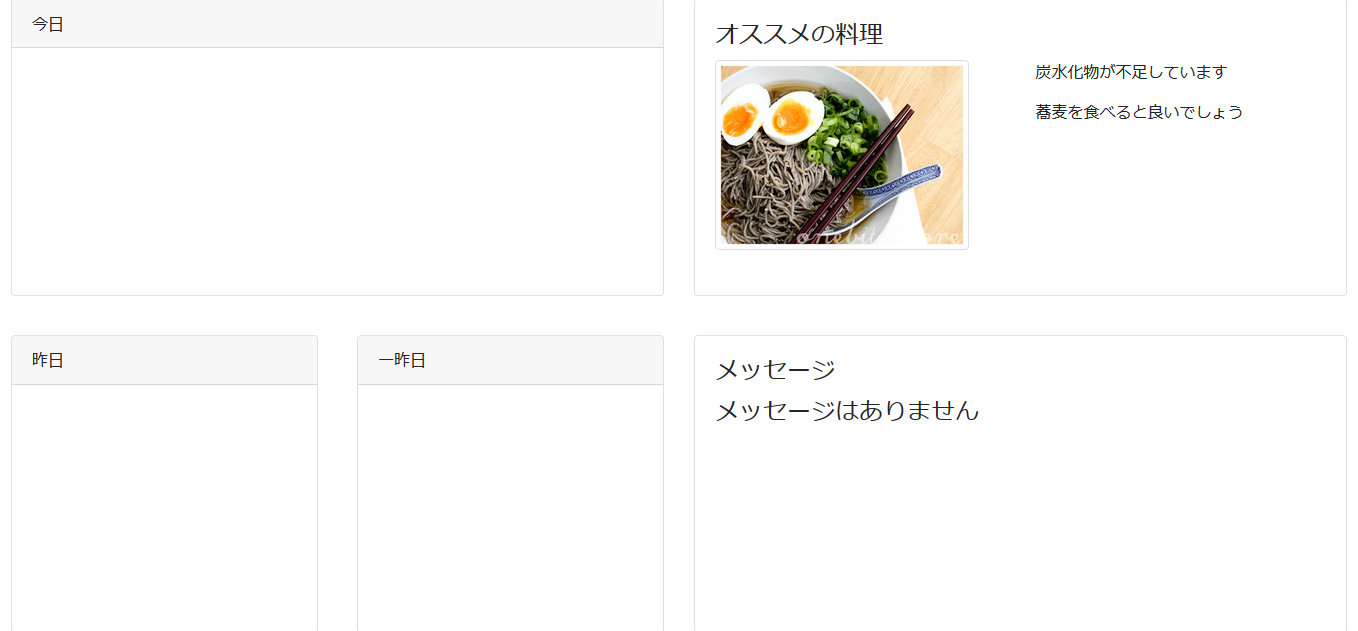
\includegraphics[width=10cm]{imgs/5_tv.png}
        \caption{テレビ画面}
        \label{fig:tv-all}
    \end{center}
\end{figure}
\bunseki{山根春貴}

\subsubsection{写真表示機能}
ボックスで自動撮影された写真が表示される.「一昨日」, 「昨日」, 「今日」の3日分の料理の写真が表示される(図\ref{fig:tv-days}).
「今日」の欄には6枚の写真, 「一昨日」と「昨日」の欄には写真が4枚, 一度に見ることができるようになっている.
\begin{figure}[htbp]
    \begin{center}
        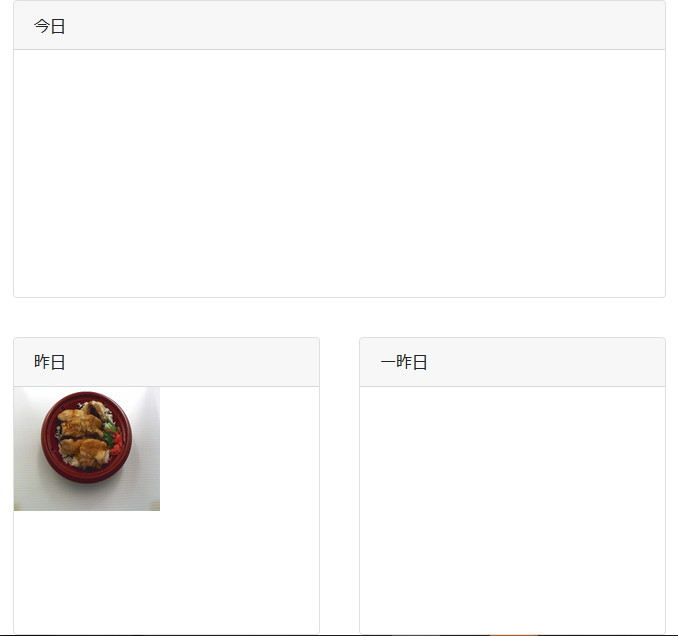
\includegraphics[width=10cm]{imgs/5_tv1.png}
        \caption{写真表示機能}
        \label{fig:tv-days}
    \end{center}
\end{figure}
\bunseki{山根春貴}

\subsubsection{オススメの料理提案機能}
ボックスで撮影された写真を1ヶ月分分析し, 平均基準値に満たない栄養素とその栄養素を補えるようなオススメの料理を提案してくれるようになっている(図\ref{fig:tv-suggestion}).
\begin{figure}[htbp]
    \begin{center}
        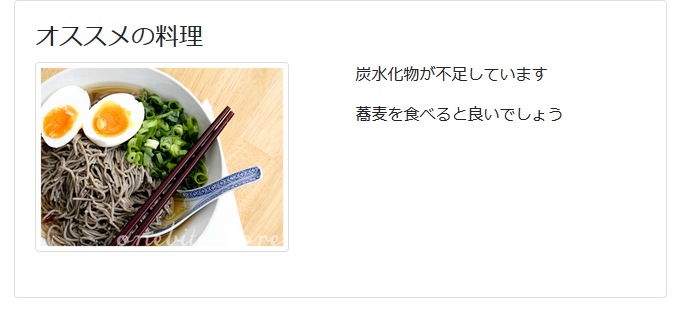
\includegraphics[width=10cm]{imgs/5_tv2.png}
        \caption{オススメ料理提案機能}
        \label{fig:tv-suggestion}
    \end{center}
\end{figure}
\bunseki{山根春貴}

\subsubsection{メッセージ機能}
Web画面から送信されたメッセージを確認することができる(図\ref{fig:tv-message}).
メッセージが届いた時に誰からメッセージが届いたのか分かるようになっている.
\begin{figure}[htbp]
    \begin{center}
        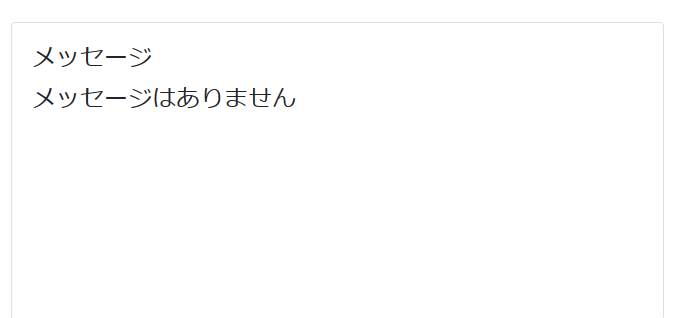
\includegraphics[width=10cm]{imgs/5_tv3.png}
        \caption{メッセージ機能}
        \label{fig:tv-mesasge}
    \end{center}
\end{figure}
\bunseki{山根春貴}
\end{document}
